% Kopfzeile beim Kapitelanfang:
\fancypagestyle{plain}{
%Kopfzeile links bzw. innen
\fancyhead[L]{\calligra\Large Vorlesung Nr. 15}
%Kopfzeile rechts bzw. außen
\fancyhead[R]{\calligra\Large 29.11.2012}
}
%Kopfzeile links bzw. innen
\fancyhead[L]{\calligra\Large Vorlesung Nr. 15}
%Kopfzeile rechts bzw. außen
\fancyhead[R]{\calligra\Large 29.11.2012}
% **************************************************
%
\wdh
$\C=\R^2$ mit 
$$(x,y)+(x',y')=(x+x',y+y')$$
$$(x,y)·(x',y')=(x·x'-y·y',x·y'-y·x')$$
$$(x,y)=x+i·y\qquad i=(0,1)\qquad i^2=(-1)$$
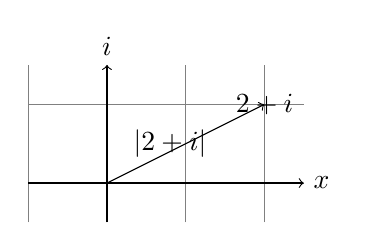
\begin{tikzpicture}[domain=-1:2.5]
    \draw[very thin,color=gray] (-1,-0.5) grid (2.5,1.5);
    \draw[->] (-1,0) -- (2.5,0) node[right] {$x$};
    \draw[->] (0,-0.5) -- (0,1.5) node[above] {$i$};
    \draw node at(2,1) {$2+i$};
    \draw node at (0.8, 0.5) {$|2+i|$};
    \draw[->] (0,0) -- (2,1);
\end{tikzpicture}
$$z=x+i·y \eC\ \Rarr\ Re(z)=x \quad Im(z)=y$$
$\overline{z}=x-i·y$
$$z·\overline{z}=(x+i·y)(x-i·y)=x^2-(i·y)^2=x^2-i^2·y^2=x^2·y^2$$
Abstand von 0 nach $z$ ist:
$$|z|=\footnote{Betrag von $z$}\sqrt{x^2+y^2}=\sqrt{z·\ol{z}}$$
$$|2+i|=\sqrt{2^2+1^2}=\sqrt{5}$$
Berechnung von $z^{-1}$\\*
$$\frac{1}{z} = \frac{\overset{\underset{↓}{reelle\ Zahl}}{z}}{\ol{z} \cdot z}$$ % Pfeil auf z {Reelle Zahl}
$$\frac{1}{2+i} = \frac{2 - i}{(2+i)(2-i)} = \frac{2-1}{5} = \frac{2}{5} = \frac{i}{5}$$

\sS{Lemma}
Sei $z,w\eC$ dann gilt:
\begin{enumerate}
\item{$\ds \ol{zw}=\ol{z}·\ol{w},\ \ol{z+w}=\ol{z}+\ol{w}$}
\item{$\ds z+\ol{z}=2 Re(z),\ z-\ol{z}=2i·Im(z)$\\*
$Re(z)=\frac{z+\ol{z}}{z}\qquad Re(z)=\frac{z-\ol{z}}{2i}$}
\end{enumerate}
%
\bew
\begin{enumerate}
\setcounter{enumi}{1}
\item{\alg{z&=x+i·y\\*
z+\ol{z}&=(x+i·y)+(x-i·y)=2x=2Re(z)\\*
z-\ol{z}&=(x+i·y)-(x-i·y)=2iy=2i·Im(z)}}
\setcounter{enumi}{0}
\item{\alg{z &= x+iy,\ w = a + ib\\*
\ol{z+w} &= \ol{x+iy + a + ib} = \ol{x+a + i(y+b)} = x + a - i(y + b) = (x - iy)+(a-ib) = \ol{z} + \ol{w}\\*
\ol{zw} &= \ol{(x+iy)(a + ib)} = \ol{(ax - by) + i(ay + bx)} = (ax - by) - i(ay + bx) = |x|\\*
\ol{z} \cdot \ol{w} &= \ol{(x+iy)} \cdot \ol{(a+ib)} = (x-iy) \cdot (a+ib) = ax - (-y)(-b) + i(a \cdot (-y) + (-b) \cdot x)\\*
&= ax - by -i(ay + bx) =  |x|}}
\end{enumerate}
\bem
Aus 3) folgt: \\*
$$z = x+iy\ \Rarr\ |z| \leq |iy| = |x| + |y|$$
Erinnerung:\\*
$$|z| \leq |x|,\ |z| \leq |y| \text{ (aus der NR)}$$

\uS{Folgen und Reihen komplexer Zahlen}

\sS{Definition (Grenzwert)}
Sei $(c_n)_{n\geq 0}$ eine Folge komplexer Zahlen, $c \in \C$\\*
Die Folge $c_n$ konvergiert gegen $c$ wenn gilt:\\[4pt]
Für jedes $\e > 0$ gibt es ein $N \in \N$, so dass für jedes $n \geq \N$ gilt $|c - c_n| < \e$
\notat{$\ds\lim_{\nif} c_n = c$ oder $c_n \to c$ für \nif}
		
\sS{Satz}
Sei $z,w\eC$
\begin{enumerate}
\item{$|z|\geq 0$, und $|z|=0$ \equ{} $z=0$ (klar)} % hier stand ein equiv
\item{$|z·w|=|z|·|w|,\ |\ol{z}|=|z|$}
\item{$|z+w|\leq|z|+|w|$ (Dreiecksungleichung)}
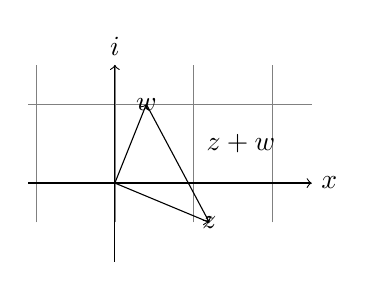
\begin{tikzpicture}[domain=-1.1:2.5]
    \draw[very thin,color=gray] (-1.1,-0.5) grid (2.5,1.5);
    \draw[->] (-1.1,0) -- (2.5,0) node[right] {$x$};
    \draw[->] (0,-1) -- (0,1.5) node[above] {$i$};
    \draw node at (0.4,1) {$w$};
    \draw node at (1.2, -0.5) {$z$};
    \draw node at (1.6, 0.5) {$z+w$};
    \draw[->] (0,0) -- (0.4,1);
    \draw[->] (0,0) -- (1.2,-0.5);
    \draw[->] (0.4,1) -- (1.2,-0.5);
\end{tikzpicture}
\end{enumerate}
\bew
\begin{enumerate}
\setcounter{enumi}{1}
\item{$\ds |z·w|=\sqrt{zw·\ol{zw}}\underset{7.3}{=}\sqrt{z·w·\ol{z}·\ol{w}}=\sqrt{z·\ol{z}·w·\ol{w}}=\sqrt{z·\ol{z}}\sqrt{w·\ol{w}}=|z|·|w|$beide reell $\geq 0$
Nachtrag rechts unten 3. tafel}
\item{\alg{|z+w|&=(z+w)·(\ol{z+w})\underset{7.3}{=}(z+w)·(\ol{z}+\ol{w})=z·\ol{z}+z·\ol{w}+w·\ol{z}+w·\ol{w}=\footnote{$\ol{z·\ol{w}}=\ol{z}·\ol{\ol{w}}=\ol{z}·w=w·\ol{z}$}z·\ol{z}+\underbrace{z·\ol{w}+\ol{z·\ol{w}}}_{2·Re(z·\ol{w})}+w·\ol{w}
&=z·\ol{z}+2·Re(z·\ol{w})+w·\ol{w}\leq |z|^2+2·|z|·|w|+|w|^2=\footnote{Für jedes $u=c+d·i\eC$ gilt $|u|=\sqrt{c^2+d^2}\geq \sqrt{c^2}=|c|=|Re(u)|$}(|z|+|w|)^2
\sqrt{}\ &\Rarr\ |z+w|=|z|+|w|\qed}}
\end{enumerate}
\bem
\begin{enumerate}
\item{Es gilt $c_n \to c\ \equ\ \ol{c_n} \to \ol{c}$}
\item{Wenn $c_n \to c$ dann $|c_n| \to |c|$}
\end{enumerate}
\bew
\begin{enumerate}
%% Er war einsam, aber schneller.
\item{$|\ol{c_n} - \ol{c}| = |\ol{c_n - c}| = |c_n - c|\ \Rarr$ Behauptung}
\item{Übung}
\end{enumerate}

\sS{Satz:}
Sei $c_n=a_n+i·b_n,\qquad c=a+ib$\\*
Es gilt $c_n→c\ \equ \ a_n→a$ und $b_n→b$
\bew
\begin{description}
\item["\Rarr"]{\desc{Es gilt:}{
$\ds |a_n-a|=|Re(c_n-c)|\leq |c_n-c|$\\*[4pt]
$\ds |b_n-b|=|Im(c_n-c)|\leq |c_n-c|$}
Also gilt: $|c_n-c|<ε\ \Rarr \ |a_n-a|<ε$ und  $|b_n-b|<ε$, somit gilt "\Rarr"}
\item["\Larr"]{Verwende $|c_n - c| \leq |a_n - a| + |b_n - b| (*)$\\*
Gegeben $\e > 0$\\*
Es gibt $N \in \N$ so dass für jedes $n \geq N$:\\
$$|a_n - a| < \frac{\e}{2}, \ |b_n - b| < \frac{\e}{2}$$
Dann gilt für $n \geq N$:\\*
$|c_n - c| \leq \frac{\e}{2} + \frac{\e}{2} = \e$\\*}
\end{description}

\sS{Definition}
Eine Folge komplexer Zahlen $(c_n)_{n\geq 0}$ heißt Cauchy-Folge, wenn für jedes $ε>0$ ein $N\eN$ existiert, so dass gilt:\\*
Für alle $n,m\geq N$ gilt $|c_n-c_m|<ε$

\sS{Satz}
Sei $c_n=a_n+ib_n$\\*
$(c_n)$ ist Cauchy-Folge \equ{} $(a_n)$ und $(b_n)$ sind Cauchy-Folgen
\bew
Genau wie Beweis von 7.6 verwende:
$$|a_n-a_m|\leq |c_n-c_m|$$
$$|b_n-b_m|\leq |c_n-c_m|$$
$$|c_n-c_m|\leq |a_n-a_m|+|b_n-b_m|$$\qed
%Satz 7.9

\sS{Satz}
Wenn $c_n→c, c'_n→c'$ konvergente Folgen komplexer Zahlen sind, dann gilt:
\begin{enumerate}
\item{$c_n+c_m→c+c'$}
\item{$c_n·c_m→c·c'$}
\item{Wenn $c\neq 0$ dann $c_n\neq 0$ für fast alle $n$ und $\frac{1}{c_n}→\frac{1}{c}$}
\end{enumerate}
\bew
Analog zum Fall reeller Folgen\qed

\sS{Definition}
Eine Reihe komplexer Zahlen\\*
$\ds\sum_{n=0}^{∞}c_n$ heißt \ul{absolut} konvergent, wenn die Reihe $\ds\sum_{n=0}^{∞}|c_n|$ konvergent ist

\sS{Satz}
Eine Folge komplexer Zahlen $(c_n)$ konvergiert \equ{} $(c_n)$ ist Cauchy-Folge
\bew
	Sei $c_n = a_n + i \cdot b_n$\\*
	$(c_n)$ konvergiert $\underset{7.6}{\equ} \ (a_n$ und $(b_n)$ konvergieren $\equ \ (a_n)$ und $(b_n)$ sind Couchy-Folgen $\underset{7.8}{\equ}$ $(c_n)$ ist Cauchy-Folge \qed

\sS{Satz}
Sei $c_n\eC$ für \nN\\*
\begin{enumerate}
\item{Majorantenkriterium:\\*
Wenn reelle Zahlen $a_n$ existieren, so dass $|c_n|\leq |a_n|$ und $\sum a_n$ konvergiert, dann konvergiert auch $\sum c_n$ absolut}
\item{Quotientenkriterium:\\*
Wenn eine reelle zahl $b\eR$ existiert mit $0\leq b<1$, so dass $|c_{n+1}\leq b·|c_n|$ für fast alle \nN\\*
Dann konvergiert $\ds\sum_{n\geq 0} c_n$ absolut}
\end{enumerate}

\sS{Satz}
Seien $\sum c_n$ und $\sum d_n$ zwei konvergente Reihen komplexer Zahlen, $\sum c_n=c,\ \sum d_n=d$\\*
Wenn eine der Reihen absolut konvergiert, konvergiert auch das Cauchy-Produkt mit Grenzwert $c·d$

\sS{Satz}
Wenn die Reihe $\sum_{n = 0}^{\infty} c_n$ absolut konvergent ist, dann ist die konvergent.
\bew
Sei $c_n = a_n + i \cdot b_n$ $$|c_n| \geq |a_n|\ \ |c_n| \geq |b_n|$$
$\sum |c_n|$ konvergent \Rarr $\sum |a|,\ \sum |b_n|$ konvergent. (Majorantenkriterium)\\*
d.h.: $\sum a_n,\ \sum |b_n|$ konvergiert absolut\\*
$\Rarr \sum a_n,\ \sum b_n$ konvergiert.\\*
$\overset{7.7}{\Rarr} \sum c_n$ konvergent \qed\\
\ul{Zusatz}\\*
Angenommen $\sum c_n$ konvergiert absolut, dann: 
$$\left| \sum_{n \geq 0} c_n \right| = \sum_{n \geq 0} c_n$$
(Dreiecksungleichung für $\infty$ viele Summanden)
\bew
Gewöhnliche Dreiecksungleichung \Rarr
$$|c_0 + c_1 + ... + c_n| \leq |c_0| + |c_1 + ... + c_n|$$
$$\text{(Partialsummen)} \leq ... \leq |c_0| + |c_1| + ... + |c_n| (*)$$
Wenn $c = \sum c_n$, dann $c = \ds\lim_{n \to \infty} (c_0 + c_1 + ... + c_n)$ (Definition des Grenzwertes einer Reihe)\\*
$\Rarr |c| = \ds\lim_{n \to \infty} |c_0 + c_1 + ... + c_n| = \left| \sum_{n = 0}^{\infty} c_n \right| \leq \lim_{n \to \infty} |c_0| + |c_1| + ... + |c_n| = \sum_{n = 0}^{\infty} |c_n|$